\chapter{はじめに}

ソフトウェア開発が大規模化する状況において,コード品質の担保や開発速度の維持は重要な課題である.
静的型付けの手法はこの課題に対処するための手段として広く用いられている.
Web 開発においては長い間 JavaScript が主要な開発言語として用いられてきたが,近年の大規模化する Web 開発においては静的手法の欠如が問題となった.

TypeScript は,動的型付けシステムである JavaScript に静的型システムによる検査を部分的に導入できるプログラミング言語であり,gradual typing システムであるとされる.
一方で,Siek らは動的型付けと静的型付けの融合を図るシステム全般が無闇に gradual typing を名乗ることを疑問視して,gradual typing システムが満たすべき基準を提案した.

本研究では,この基準に照らして TypeScript が gradual typing の条件を満たすようなコンパイラを実装する.

\section{背景}

\subsection{TypeScript}

TypeScript は,Microsoft により開発されているプログラミング言語である.
TypeScript は ECMAScript 5\cite{ES5}を拡張した構文を持ち,既存の構文に型アノテーションを追加できる.
また,それを補助するものとして,型エイリアスや関数オーバーロードを宣言する機能も用意されている.
TypeScript コンパイラは型アノテーション及び型推論機構を基に TypeScript プログラムを静的に検査し,プログラムのある種の誤りを検出する機能を持つ.

TypeScript の最も大きな特徴のひとつは\texttt{any}型の存在だ.
ある値が\texttt{any}型を持つ場合,その値に対する一切の操作は TypeScript コンパイラによるチェックの対象とならない.
特に,潜在的に危険な操作であっても\texttt{any}型を用いることで型検査を成功させることができる.
これは時として,型情報と矛盾する挙動を実行時に引き起こしたり,実行時エラーという結果に繋がったりする.

TypeScript に\texttt{any}型が存在する理由は,型をオプショナルなものとするためである.
ここで,オプショナルというのは,プログラム全体を型検査しなくてもよいということを指していると考えられる.
実際,TypeScript ではあらゆる型アノテーションが省略可能だ.
TypeScript コンパイラは原則として,型アノテーションが提供されているところや,型アノテーションが無くても型を推論可能なところのみを型検査の対象とする.

このような「型アノテーションが存在するところのみを型検査の対象とする」という挙動を,静的型付け\footnote{あるいは静的型システム}の枠組みで表現するための道具が\texttt{any}型である.
TypeScript コンパイラは型アノテーションが存在しない変数を\texttt{any}型として扱うことで,その変数が関わる部分の型検査を実質的に無効化する.
そもそも,TypeScript コンパイラの型推論においては,変数の型は原則として宣言時に決定される.
これは Hindley-Milner 型推論\cite{MILNER1978348}のような,変数の使われ方から型を推論できる方法とは大きく異なる特徴である.
関数の引数も例外ではなく,一部の場合\footnote{contextual typeにより型が推論可能な場合など}を除いて,引数の型は明示的に宣言しなければならない\footnote{多相関数も明示的に型引数を宣言しなければならない}.
それにも関わらず変数や引数の型アノテーションが省略された場合,TypeScript コンパイラはその変数の型の情報を得られない状態となる.
TypeScript はこのような場合にその変数の型を\texttt{any}とすることで解決するというデザインを採用している.
それ以外にも,変数の型が推論できないさまざまな場面において\texttt{any}型が当てはめられる.

この特徴により,TypeScript は JavaScript からの移行を支援している.
そもそも,ただの JavaScript プログラムは,型アノテーションが完全に省略された TypeScript とみなすことができる.
この状態から徐々に型アノテーションを追加することによって,TypeScript による型検査が行われる部分を段階的に増やすことが可能だ.
この段階において,TypeScript プログラムは型検査が行われる部分と行われない部分が混在している状態となる.

\subsection{Gradual Typing}

Gradual typing \cite{GradualTyping}は,Siek と Taha が 2006 年に提案した,静的型付けと動的型付けを融合させる手法のひとつである.
静的型付けと動的型付けは異なる利点と欠点を持つものとして共存してきたものであり,両方の手法を取り入れる方法も古くから模索されてきた.
Gradual Typing ではこれら 2 つの方式をひとつのプログラムの中に共存させることができる.
特に,プログラマがアノテーションを用いて,プログラムのどこに静的な検査を適用できるという特徴を持つようなシステムが Gradual Typing と呼ばれる.
当該論文では,特に関数型言語に対して Gradual Typing の要件を満たす型システムを提案している.

Siek と Taha の型システムでは,通常の型に加えて\texttt{?}型が導入されてる.
\texttt{?}型が与えられた変数は静的なチェックが行われない.
その点で,これは静的型検査の対象としないというアノテーションを表す型と見なすことができるものであり,TypeScript の\texttt{any}型に相当する.

\section{Siek と Taha の体系の型安全性}
\label{sec:safety_of_siek_taha}

Gradual Typing においては,プログラムの正しさを静的に保証することは当然ながらできない.
型によって静的な検査を無効化した隙に誤りが入りこむかもしれないからである.
Siek と Taha の論文の序盤から例を引用する.

\begin{quote}
    ((λ (x) (succ x)) \#t)
\end{quote}

これは彼らが提案した計算体系$\lambda^?_\to$の式だが,TypeScript に直すと以下に相当する.

\begin{lstlisting}[caption={TypeScript における例}, label={lst:example_ts}]
const succ = (x: number) => x + 1;

((x: any) => succ(x))(true)
\end{lstlisting}

\ref{lst:example_ts}の式は,実行すると\texttt{true}という\texttt{boolean}型の値が\texttt{succ}関数に渡される.
\texttt{succ}は\texttt{number}型の引数を渡すべきなので,これは誤ったプログラムということになる.

ただし,上の式は型システムによる静的検査をくぐり抜ける.
これは,\texttt{x}という\texttt{?}型\footnote{\texttt{any}型}を持つ変数を経由しているからである.
変数\texttt{x}に値が入った時点で,型システム上ではその値が本来何型であるかという情報は消えている.
また,\texttt{?}型はどのような型としても使用できることから,\texttt{number}型を受け取る関数\texttt{succ}に\texttt{x}を渡しても問題ない.

Siek と Taha の体系$\lambda^?_\to$においては上記のように誤ったプログラムはどのような結果になるだろうか.
実はこの体系ではランタイムに誤りを検知する.
これは,キャストの情報を値に保存するセマンティクスによって実現される.

Gradual typing においては\texttt{?}型の存在が注目されるが,それに加えてランタイムのチェックを合わせてひとつの理論であるということは強調するに値する.

この体系では,プログラムの意味は別の体系$\lambda^{<\tau>}_\to$のプログラムへの変換を通して理解される.
上記のプログラムは以下のように変換される.

\begin{quote}
    ((λ (x : ?) (succ <number>x)) <?>\#t)
\end{quote}

元々のプログラムとの違いは,\texttt{<number>x}や\texttt{<?>}のように値の前に型が書かれている部分がある点である.
このような式はキャスト式と呼ばれる.
このプログラムでは,「\texttt{boolean}型の値を\texttt{?}型として使う」や「\texttt{?}型の値を\texttt{number}型として使う」といった操作がキャスト式によって明示的に表現されている.

上のプログラムを実行すると,変数\texttt{x}に\texttt{<?>\#t}が入るので,\texttt{<number>x}は\texttt{<number><?>\#t}という値になる.
\texttt{\#t}が\texttt{boolean}型であることに留意すると,ここで\texttt{boolean}型から\texttt{number}型へのキャストが発生していることが明らかになる.
これは誤りなので,ここでランタイムエラーが発生する.

当該論文では,彼らの体系の“型安全性“の証明が与えられている.
\texttt{?}型の存在により型の誤りがランタイムに発生することは避けられないが,それは全て上述の CastError としてキャッチされる.
ここでの型安全性は,上述のランタイム機構をすり抜ける型の誤りが発生しないという意味で用いられている.
実際,上記で説明した通り,型アノテーションに反する値がランタイムに発生することはない.

\section{Criteria for Gradual Typing}

前述の論文以降 gradual typing という言葉は知名度を増したが,その結果として gradual typing という言葉が何を指しているのか曖昧になり,静的型付けと動的型付けを融合させる試みが無秩序に gradual typing を名乗るという問題があった.
Siek ら\cite{siek_et_al:LIPIcs.SNAPL.2015.274}の 2015 年の論文はこの問題を指摘し,gradual typing を名乗るシステムの条件を整理した.

Gradual typing システムが満たすべき条件は以下の通りだ(論文の Theorem 1 から 5).
2006 年のオリジナルの体系はこれらの条件を全て満たすことが示されている.

\begin{enumerate}
    \item 静的型付けの体系を内包する.すなわち,全ての型がアノテートされている\footnote{\texttt{?}型を用いない}プログラムは,ただの静的型付けシステムと同じ挙動をする\footnote{静的検査の結果も,実行結果も同じである}.
    \item 動的型付けの体系を内包する.すなわち,型アノテーションが無い\footnote{全ての型が\texttt{?}である}プログラムはただの動的型付けシステムと同じ挙動をする.また,任意の式の型が\texttt{?}である.
    \item 健全性.前節で述べたように,ランタイムにキャッチできない型の誤りは発生しない.
    \item Blame-Subtyping Theorem.$T_1 <: T_2$ならば,$T_1$から$T_2$へのキャストはランタイム型エラーの原因とならない.
    \item Gradual Guarantee.すなわち,静的型検査に成功するプログラムから型アノテーションを減らしても静的型検査は成功し,型も変わらない.また,プログラムから型アノテーションを減らしても動作が変わらない\footnote{ただし,キャッチできるランタイム型エラーが減る可能性はある}.
\end{enumerate}

なお,4. に出てくる部分型関係は以下のように定義されている(前述の論文\cite{siek_et_al:LIPIcs.SNAPL.2015.274}から引用).
この論文では今まで\texttt{?}型と呼んでいたものが$*$型となっている.
なお,$*$というのは基本型または$* \to *$である.

\[
    \begin{array}{ccc}
        B <: B                & \quad          & * <: *                                                         \\[1em]
        \frac{T <: G}{T <: *} & \quad          & \frac{S_1 <: T_1 \quad T_2 <: S_2}{T_1 \to T_2 <: S_1 \to S_2} \\[2em]
                              & \boxed{T <: T} &
    \end{array}
\]

この定義からは$number \to *$や$* \to number <: number \to number$,また$* \to number <: *$などが成り立つ.
一方,$number \to * <: *$のようなものは成り立たない.

部分型関係における$*$の扱いは注目に値する.
特に,$* <: T$となる$T$は$*$だけである.$*$は静的解析において型エラーの原因にはならないが,ランタイム型エラーの原因となる,
それゆえ,特に上述の定理 4 の観点からは他の型の部分型とはなれない.

\section{TypeScriptの型システム}

TypeScript の型システムは,完全に静的なシチュエーションにおいても健全性を持たないことが広く知られている.

静的型検査の側面において,TypeScript の\texttt{any}型は Siek と Taha の gradual typing 型システムにおける\texttt{?}型と同じ特徴を持つ.
すなわち,\texttt{any}型の値は他の任意の型の値が必要な場面において使用可能である.
また,\texttt{any}型が求められる場面においても任意の型の値を\texttt{any}型として使用できる.

一方で,TypeScript のランタイムの挙動は$\lambda^?_\to$とは大きく異なる.
具体的には,ランタイムの型チェックが行われない.
そもそも,TypeScript には型の情報によってランタイムの挙動が変化しないという大原則があるため,\ref{sec:safety_of_siek_taha}で説明したような型情報ベースのランタイム型チェックは趣旨に沿わない.
このようなデザインを取っている理由として,型システムによるランタイムのオーバーヘッドを避けることが第一に挙げられる.
また,型によるランタイムの挙動への影響を排除することで,JavaScript ユーザーから見て TypeScript のコンパイル処理の透明性を向上するという目的があると推測される.

上記の理由から,\texttt{any}型の存在に起因する型のミスマッチは,$\lambda^?_\to$における CastError のような形でキャッチされるのではなく,別の予期せぬ形で現れることとなる.
これは,TypeScript の型システムでは,gradual typing の意味での健全性が失われていることを意味する.

以降でもランタイム型エラーという語を用いるが,これは gradual typing システムによるランタイムのチェックによって検出されるものを指す.
実際の TypeScript では,型のミスマッチは呼びだそうとしたメソッドが存在しないことによる実行時エラーや,\texttt{undefined}や\texttt{null}に対するプロパティアクセスしたことによる実行時エラーなど,その結果はさまざまな形で現れる.
以降では,これらは前述のランタイム型エラーとは区別し,予期せぬ結果と呼んでいる.
ランタイム型エラーはプログラムの動的な部分のチェックが正しく行われた結果として現れるのに対し,予期せぬ結果は,システムの健全性が失われた結果として現れるものである.

\subsection{TypeScriptとCriteria for Gradual Typing}

TypeScript の型システムの性質を Siek らの criteria for gradual typing に照らし合わせてみる.

1(静的型付けの体系を内包する)と 2(動的型付けの体系を内包する)については成り立つ.
というよりも,1 と 2 は変なセマンティクスを持つ体系を除外するための条件であると考えられるので,これらの条件は今回の設定ではあまり意味を持たない.
1 に関しては TypeScript と比較するための静的なシステムが必要だが,それは\texttt{any}を取り除いた TypeScript そのものである.

2 については比較対象の動的システムは JavaScript となるが,上述の性質から 2 が成り立つことは明らかである.
ただし,この条件を TypeScript に当てはめる際には注意すべき点がある.
本来の TypeScript では「任意の式の型が\texttt{any}型である」は満たされない.
例えば次のプログラムにおいて変数\texttt{v}は\texttt{number}型である.

\begin{lstlisting}
const x: any = 123;
const y: any = 456;
const v = x * y;
\end{lstlisting}

しかしながら,これは\texttt{*}演算子の挙動によるものである.
Siek らが本来対象としているのが関数型言語であることを鑑みると,\texttt{*}のような計算も全て関数としてみなすのが適切である.
Siek らの論文にも,2 の条件については組みこみ定数や関数も全て$*$型として見なすものと定義されている.
実際,このことをより忠実に反映した以下の TypeScript プログラムでは変数\texttt{v}の型は\texttt{any}となる.

\begin{lstlisting}
const mul: any = (x: any, y: any) => x * y;
const x: any = 123;
const y: any = 456;
const v = mul(x, y);
\end{lstlisting}

3 つ目の条件である健全性については,すでに議論した通り,明らかに満たされない.
そもそもランタイムのチェックがまったく行われないからである.

4 についても状況設定から議論する必要がある.
部分型からのキャストはランタイム型エラーの原因にならないという条件だが,そもそも全くランタイムの型チェックが行われない設定では意味のある主張ではない.
一方で,その他の予期せぬ結果もここでのエラーに含めることも考えられる.
ただし,その場合は健全性が失われていることから反例を作るのは簡単である.

最後の条件,gradual guarantee については,TypeScript の言葉で言い換えれば,型アノテーションを減らすというのは型註釈を何らかの型から\texttt{any}に変えることを指す.
ランタイムの動作については,前述の性質から型註釈が\texttt{any}に変わってもランタイムの動作が変わらないことは自明である.
一方で,静的型検査については自明でない.

以上の 5 条件について議論した結果において,TypeScript が gradual typing の意味での健全性を失っていることが特徴として現れている.
ランタイムの型チェックを行わないことは TypeScript の根本的な言語デザインであり,その点において gradual typing とは乖離していることが分かった.

\subsection{Safe TypeScriptにおける対応}
\label{sec:safe_typescript}

前節では,TypeScript が gradual typing の意味において健全性を持たないことで gradual typing の基準を満たしていないことを指摘した.
この問題に対応するアイデアのひとつが Safe TypeScript\cite{rastogi2015safe}である.
これは,健全性を保ったバージョンの TypeScript として Microsoft Research により開発されたものである.

Safe TypeScript が健全性を得るために行なった変更は大きく分けると 2 つある.
1 つは型システムへの変更により静的検査における健全性を確保することであり,もう 1 つはランタイム型チェックの導入により gradual typing の意味での健全性を確保することである.
実際の論文では,ランタイム型チェックのオーバーヘッドを削減するための工夫が述べられており,それらによってランタイム型チェックのオーバーヘッドが 15\%程度に抑えられたことが報告されている.

ランタイム型チェックの一例が下の図に現れている(当該論文\cite{rastogi2015safe}から引用).
関数\texttt{f}の返り値である\texttt{x.f}が本当にアノテーション通りの\texttt{number}型であるかどうかランタイムにチェックするための\texttt{RT.check}という呼び出しが追加されていることが分かる.

\begin{figure}[H]
    \centering
    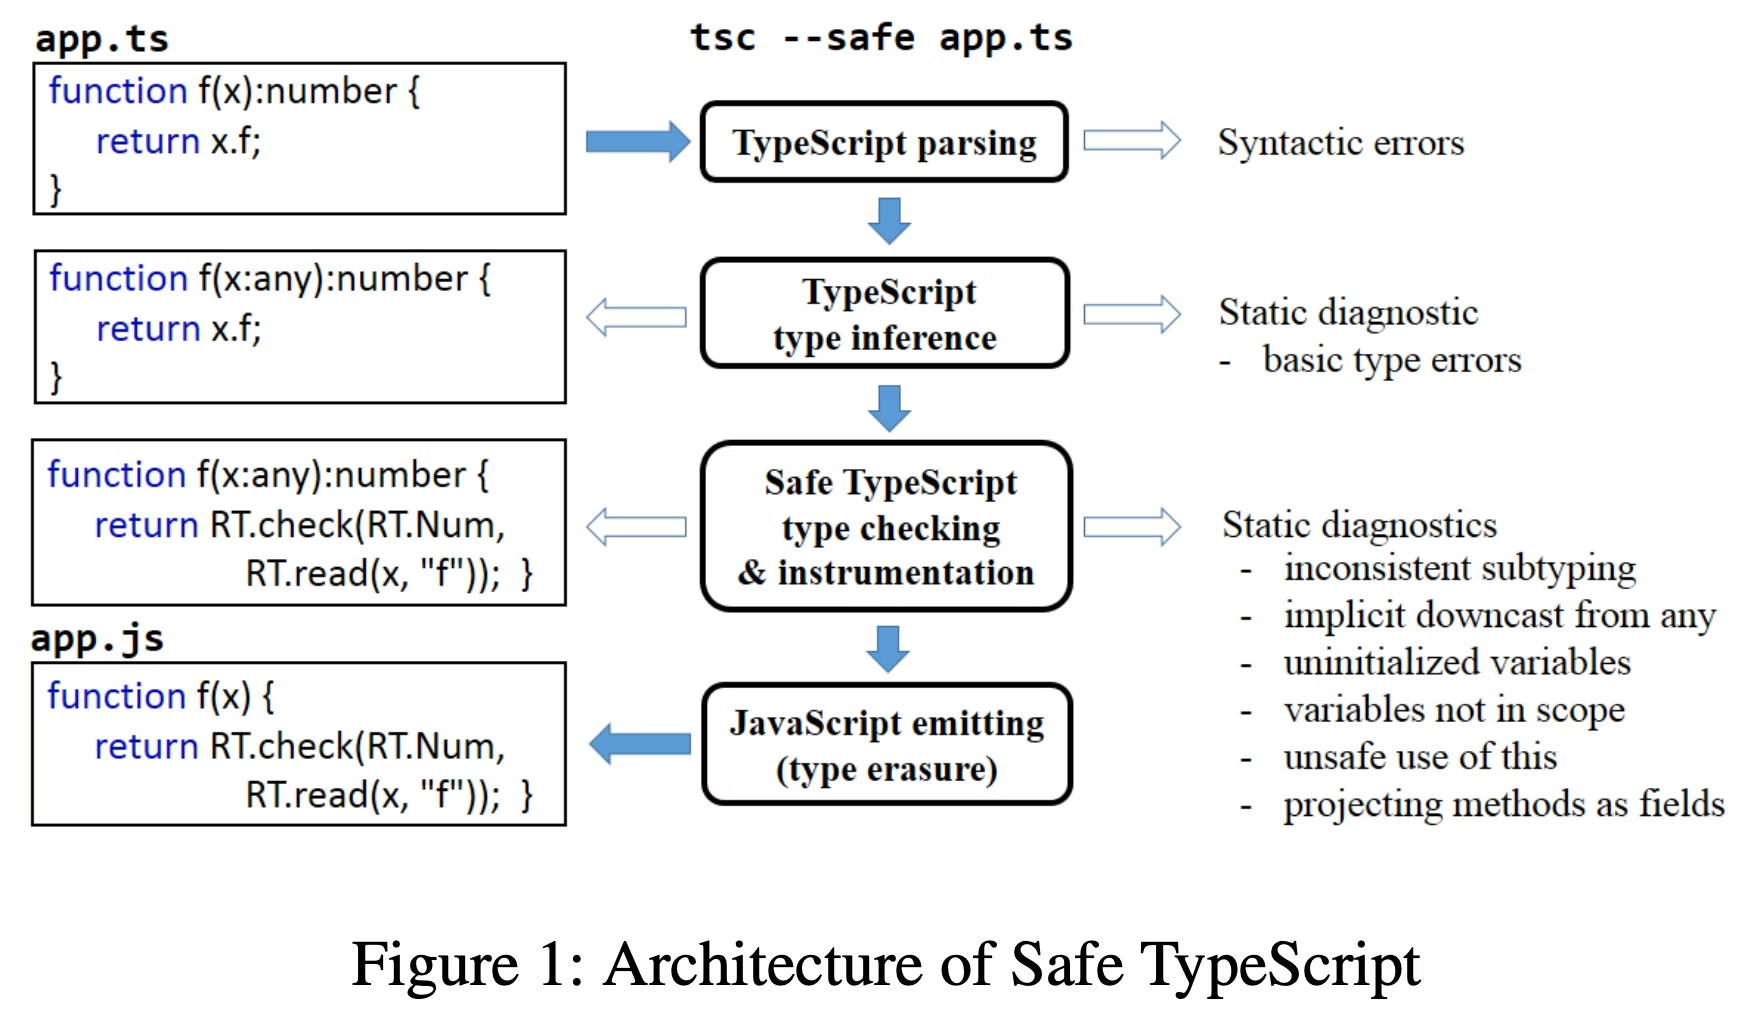
\includegraphics[width=0.8\textwidth]{figures/fig_overview_safe_typescript.png}
    \caption{Safe TypeScriptにおけるランタイム型チェックの例}
\end{figure}

Safe TypeScript は明確に gradual type system を名乗っている.
実際,論文で主張されている通り Safe TypeScript は gradual typing の意味での健全性を備えている.

しかし,Safe TypeScript ではオーバーヘッドを減らす様々な工夫をしてもなお,15\%のオーバーヘッドが存在する.

\section{本研究の目的}

\ref{sec:safe_typescript}で述べた通り,Safe TypeScript は gradual typing の意味での健全性を持つことができる.
Safe TypeScript は筋こそはいいが,ランタイムのオーバーヘッドが大きいという問題がある.

現代の Web 開発において,TypeScript は JavaScript へトランスパイルされ,ブラウザで実行される.
ランタイムのオーバーヘッドはユーザビリティに大きな影響を与える.
そのため,Safe TypeScript は実用的な選択肢とは言い難い.

開発者の求める TypeScript の使用方法と,gradual typing は相反していると筆者は考える.
開発者は TypeScript を使うことで,JavaScript のような柔軟性を持ちつつ,静的型検査による安全性を得たいと考えている.

ここで,JavaScript の柔軟性を「型アノテーションが不要である」という意味で捉えると,従来の TypeScript では \texttt{any}型となる部分が柔軟性を持つ部分であると言える.
しかし,開発者が TypeScript に求める本当の柔軟性は省略された型アノテーションを補完した上での静的型検査による安全性である.

そこで,TypeScript の型システムを拡張し,型解析を通して健全性を保つことを目指す新しい TypeScript 型検査機「decaf」を提案する.
